\documentclass{article}

\usepackage[spanish]{babel}
\usepackage{listings}
\usepackage{color}
\usepackage[numbers,sort&compress]{natbib}
\usepackage{graphicx}
\usepackage{subfigure}
\usepackage{url}
\usepackage{amsmath}
\usepackage{hyperref}
\usepackage[top=15mm, bottom=40mm, left=15mm, right=15mm]{geometry}
\setlength{\parskip}{2mm}
\setlength{\parindent}{0pt}

\setlength{\parskip}{2mm}
\setlength{\parindent}{0pt}
\definecolor{blue}{rgb}{0,0.6,0}
\definecolor{gray}{rgb}{0.3,0.3,0.3}
\definecolor{orange}{rgb}{0.8,0.4,0}
\definecolor{mostaza}{rgb}{0.9,0.8,0.1}

\lstset{ %
  language=R,                     % the language of the code
  basicstyle=\footnotesize,       % the size of the fonts that are used for the code
  numbers=left,                   % where to put the line-numbers
  numberstyle=\tiny\color{gray},  % the style that is used for the line-numbers
  stepnumber=1,                   % the step between two line-numbers. If it's 1, each line
                                  % will be numbered
  numbersep=5pt,                  % how far the line-numbers are from the code
  backgroundcolor=\color{white},  % choose the background color. You must add \usepackage{color}
  showspaces=false,               % show spaces adding particular underscores
  showstringspaces=false,         % underline spaces within strings
  showtabs=false,                 % show tabs within strings adding particular underscores
  frame=single,                   % adds a frame around the code
  rulecolor=\color{black},        % if not set, the frame-color may be changed on line-breaks within not-black text (e.g. commens (green here))
  tabsize=2,                      % sets default tabsize to 2 spaces
  captionpos=b,                   % sets the caption-position to bottom
  breaklines=true,                % sets automatic line breaking
  breakatwhitespace=false,        % sets if automatic breaks should only happen at whitespace
  title=\lstname,                 % show the filename of files included with \lstinputlisting;
                                  % also try caption instead of title
  keywordstyle=\color{orange},      % keyword style
  commentstyle=\color{blue},   % comment style
  stringstyle=\color{mostaza},      % string literal style
  escapeinside={\%*}{*)},         % if you want to add a comment within your code
  morekeywords={*,...}            % if you want to add more keywords to the set
} 

\author{1445183}
\title{Frentes de Pareto}
\date{\today}

\begin{document}

\maketitle

\section{Objetivo}
Paralelizar el código y graficar el porcentaje de soluciones de Pareto como función del número de funciones objetivo, verificando que las diferencias observadas sean estadísticamente significativas.

\section{Descripción}
Se empieza paralelizando el código proporcionado por la práctica \cite{elisaweb11} desde el inicio.
\begin{lstlisting}[language=R]
library(doParallel)
cluster <- makeCluster(detectCores() - 1)
pick.one <- function(x) {
  if (length(x) == 1) {
    return(x)
  } else {
    return(sample(x, 1))
  }
}
[...]
\end{lstlisting}

Después el código es modificado para que sean \texttt{100} soluciones aleatorias (\textit{n}), con funciones objetivo (\textit{k}) de \texttt{2} a \texttt{8} con \texttt{25} réplicas cada uno haciendo uso de \texttt{for}.

\begin{lstlisting}[language=R]
vc <- 4
md <- 3
tc <- 5
n=100
datos<-data.frame(funciones= integer(), replicas=integer(), 
                  soluciones= integer(), porcentaje=integer())

for(k in 2:8){
  print(k)
  for(replica in 1:25){
    print(replica)
    obj <- list()
    for (i in 1:k) {
      obj[[i]] <- poli(vc, md, tc)
    }
    minim <- (runif(k) > 0.5)
    sign <- (1 + -2 * minim)
    sol <- matrix(runif(vc * n), nrow=n, ncol=vc)
    clusterExport(cluster, c("n","k", "sol", "tc", "obj", "eval", "dim", "valor"))
\end{lstlisting}

Para las pruebas estadísticas se hizo uso de \texttt{Shapiro.test} y \texttt{Dunn.test} para este último se tuvo que instalar el paquete en \texttt{R}.

\section{Resultados}

Se puede observar en la figura \ref{fig1} los porcentajes obtenidos para cada función objetivo (\textit{k}), donde a mayor cantidad de \textit{k} los porcentajes tienden a ser mayores.

\begin{figure}[htbp]
\centering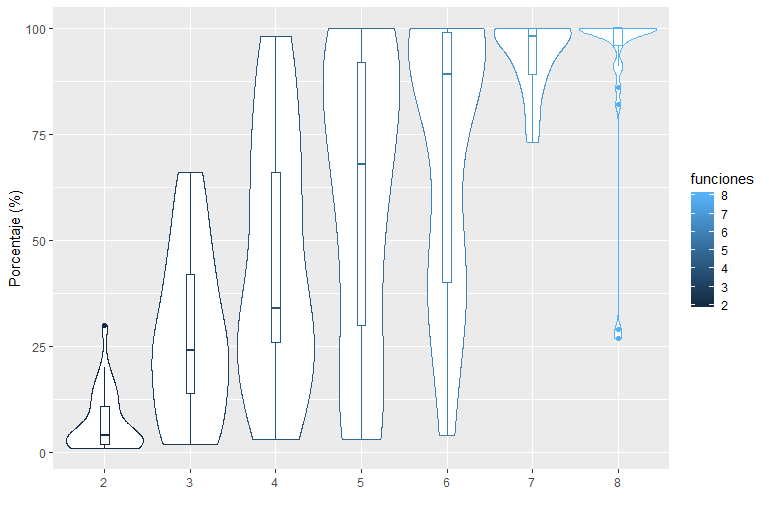
\includegraphics[width=160mm]{violin11.png}
\caption{porcentaje de las funciones objetivo  (\textit{k}})
\label{fig1}
\end{figure}

La prueba de \texttt{shapiro.test} nos da el valor \textit{p} que en este caso es menor de \texttt{0.05} por lo que los datos no cumplen la normalidad, tomando de referencia el trabajo de \textit{Saus} \cite{saus} se hace la prueba \texttt{dunn.test} \cite{alexis}.

\begin{lstlisting}[language=R]
shapiro.test(datos$porcentaje)

	Shapiro-Wilk normality test

data:  datos$porcentaje
W = 0.84612, p-value = 2.668e-12
\end{lstlisting}

\begin{lstlisting}[language=R]
  Kruskal-Wallis rank sum test

data: x and group
Kruskal-Wallis chi-squared = 106.5637, df = 6, p-value = 0


                           Comparison of x by group                            
                                (No adjustment)                                
Col Mean-|
Row Mean |          2          3          4          5          6          7
---------+------------------------------------------------------------------
       3 |  -2.190205
         |    0.0143*
         |
       4 |  -3.499568  -1.309362
         |    0.0002*     0.0952
         |
       5 |  -4.787924  -2.597718  -1.288356
         |    0.0000*    0.0047*     0.0988
         |
       6 |  -5.957247  -3.767042  -2.457679  -1.169323
         |    0.0000*    0.0001*    0.0070*     0.1211
         |
       7 |  -7.877179  -5.686973  -4.377611  -3.089254  -1.919931
         |    0.0000*    0.0000*    0.0000*    0.0010*     0.0274
         |
       8 |  -8.134850  -5.944644  -4.635282  -3.346925  -2.177602  -0.257671
         |    0.0000*    0.0000*    0.0000*    0.0004*    0.0147*     0.3983

alpha = 0.05
Reject Ho if p <= alpha/2
\end{lstlisting}





\section{Conclusión}

A partir de siete objetivos se empieza a observar que los porcentajes de las soluciones no dominadas son equivalentes, es decir, que no existen diferencias significativas. Al existir mayor cantidad de objetivos la comparación entre ellos aumenta por lo que si al compararse un objetivo con otro no mejora hay más posibilidades de que con otro si, de manera que hay mayor cantidad de soluciones dominantes, esto es la frente de pareto.




\bibliographystyle{plainnat}
\bibliography{biblio}

\end{document}